\documentclass[11pt,letter]{article}
	\usepackage[english]{babel}%required allways
	\usepackage[authoryear]{natbib}
	\usepackage{float} 		% required for example and excercise styles
    %\floatstyle{plaintop}
    %\restylefloat{table}	
	\usepackage[intlimits]{amsmath}%provide option intlimits to
    \usepackage{amsfonts}
	\usepackage{graphicx} 	%required for including external graphics files
    \usepackage{amsmath}
    \usepackage{footnote}
    \usepackage{setspace}
     \usepackage{authblk}
     \usepackage{threeparttable}
     \usepackage{rotating}
     \usepackage{epstopdf}
     %\usepackage[margin=1in]{geometry}
    \usepackage[top=1.6in, bottom=1.6in, left=1.2in, right=1.2in]{geometry}
%     \usepackage{footmisc}
     \renewcommand{\thefootnote}{\fnsymbol{footnote}}
%     \usepackage{abstract}
   %  \renewcommand{\abstractnamefont}{\normalfont\Large\textbf}
    % \renewcommand{\abstracttextfont}{\normalfont}
     \newcommand{\sectionbreak}{\clearpage}
     \DeclareMathOperator*{\Max}{Max}
     \usepackage{hyperref}
     \hypersetup{colorlinks=true,citecolor=blue}
     %\renewcommand{\refname}{References}
     %\renewcommand{\bibname}{References}
	\usepackage{booktabs}
	\usepackage{subfig}
	

\title{Understanding Joint Retirement\footnote{We acknowledge financial support from the National Institute of Aging (NIA) and the Netherlands Scientific Organization of Scientific Research (NWO).}}

\makeatletter
\let\@fnsymbol\@alph
\makeatother

\usepackage[T1]{fontenc}
\usepackage{ifxetex}
\ifxetex
%% XeLaTeX
 \usepackage{fontspec}
 \usepackage{xunicode}
 \defaultfontfeatures{Mapping=text-text}
 \setsansfont{GillSans}
%  \setsansfont{Verdana}
  \renewcommand*{\familydefault}{\sfdefault}

\else
 %\usepackage{arev}
 %\renewcommand{\familydefault}{\sfdefault}
 \usepackage[utf8]{inputenc}
 \usepackage[T1]{fontenc}

\fi
\author{Pierre-Carl Michaud\thanks{HEC Montreal and NBER. Email: pierre-carl.michaud@hec.ca}\qquad Arthur Van Soest\thanks{Netspar, Tilburg University, RAND and IZA. Email: A.H.O.vanSoest@uvt.nl} \qquad Luc Bissonnette\thanks{CEB, now Gartner. Email: Luc.Bissonnette@ecn.ulaval.ca}}

%\renewcommand\Authands{ and }
\date{September 1, 2018}

\begin{document}
\maketitle
\onehalfspacing

\begin{abstract}
Evidence from different sources shows that spouses' retirement decisions are correlated. Retirement policies affecting individuals in couples are therefore also likely to affect behavior of their spouses. It is therefore important to account for joint features in modeling retirement. This paper studies a structural collective model of labor supply and retirement of both partners in a couple with interdependent preferences, imperfect knowledge of preferences of the spouse, and subjective expectations about the future. We propose a novel method to estimate preferences and the intra-household bargaining process, which relies on stated preferences data collected in the Health and Retirement Study. Respondents were asked to choose between hypothetical retirement trajectories describing the retirement ages and replacement rates of both spouses from three perspectives: considering their own preferences only, the preferences of their spouse only, or the most likely decision for the household. With these data, all model parameters are identified and potential sources of joint retirement can be disentangled. We find that males misperceive their wives' preferences, overestimating their disutility of work. Our estimates correct for this bias. They suggest that correlation in unobserved heterogeneity components of the partners' marginal utility of leisure explains a large share of joint retirement decisions. We also find significant positive complementarities in leisure, but this explains a much smaller part of joint retirement.\\

\setlength{\parindent}{0cm}
\textbf{Keywords:  Collective models, Leisure complementarity, Stated choices, Identification }

\par \textbf{JEL Codes:  D13, J26, C81}

\end{abstract}

\doublespacing
\renewcommand{\thefootnote}{\arabic{footnote}}


\newpage
\section{Introduction}

\par Population aging has led to a debate on the labor force participation of older workers, increasing the need for understanding retirement decisions and their sensitivity for policy measures. Earlier studies often only focus on the retirement behavior of males, due to the fact that women often left the labor market long before reaching retirement age. Since the labor force participation rate of women has grown substantially over the last decades, understanding their retirement decisions has gained importance. Moreover, there is clear evidence that the retirement decisions within couples are interdependent, with a significant proportion of spouses retiring at approximately the same time, irrespective of their age difference (``joint retirement''). \cite{hurd1990} already pointed out that between 20 and 30 percent of all couples retire within one year of each other. Since then, a new line of research has emerged aimed at analyzing and understanding the retirement behavior of couples. Empirical evidence of joint retirement decisions has been documented for several cohorts and countries, including \citet{blau1998} (Retirement History Study), \citet{gustman2000retirement} (National Longitudinal Survey of Mature Women), \cite{gustman2004} and \cite{casanova2010} (Health and Retirement Study), \citet{banks2007dynamics} (English Longitudinal Study of Ageing), and \citet{Hospido2013} (Survey of Health Ageing and Retirement in Europe).

\par There are several potential links between spouses' retirement decisions that may explain joint retirement. The first one operates through the household budget constraint (see \citet{blau1998}; \citet{casanova2010}). \cite{casanova2010} shows that under certain conditions, the fact that resources are shared can increase the probability of joint retirement. In addition, the spouse allowance in the US old age social security benefit system creates financial incentives that explain coordination in retirement dates (see \citet{mccarty1990}). The second channel originates from  preferences: It is plausible that spouses enjoy spending leisure time together so that the marginal utility of retirement increases when the partner is also retired (complementarities in leisure, leading to a causal effect of the retirement of one spouse on retirement of the other spouse; see \citet{gustman2000retirement,gustman2004,gustman2009}, \citet{elena2016} or \citet{michaud2011}). The third channel is the correlation in spouses' (unobserved) tastes for leisure (See \citet{gustman2000retirement,gustman2004}) that can be due to assortative matching. The literature has not come to a clear conclusion on the relative importance of these three channels, but does conclude that ignoring joint retirement may severely underestimate the overall impact of reforms in retirement policy. For example, \citet{coile2004} finds that neglecting the spill-over effect on the behavior of the spouse may underestimate the overall impact of a typical policy by 13\% to 20\%.

\par To model joint behavior, the collective model empirically outperforms the neo-classical unitary model assuming that each household behaves as a single decision maker, both for consumption and labor supply behavior (\citet{fortin1997}, \citet{bourguignon1993}, \citet{cherchye2009}). The collective model (\citet{chiappori1988}) starts from the basic assumption that in a multi-person household, household members have their own utility functions but cooperate in some bargaining process that results in a Pareto-efficient allocation. The assumption of cooperation seems quite natural, given that spouses interact very often.\footnote{\citet{gustman2000retirement} and several follow-up studies estimate a structural retirement model of joint retirement assuming noncooperative behavior and Nash bargaining.} Several studies found support for the collective model in the sense that its theoretical implications cannot be rejected when tested on multi-person household data (\citet{chiappori2002}, \citet{cherchye2009}). Yet, some assumptions of that model remain untested. In particular, it is assumed that each spouse knows the preferences of the other spouse and therefore can correctly pick a Pareto optimal outcome. To the best of our knowledge, no study has tested this assumption.

\par A major challenge of the collective model is the identification of parameters in a realistic context with externalities and public goods. Additional identifying assumptions are usually needed in order to estimate the model and test its validity. \citet{chiappori1988,chiappori1992} shows that if preferences are egoistic, the usual data on actual household choices are enough to identify the sharing rule up to a constant. The assumption of egoistic preference, however, is rather restrictive in the context of retirement, since it means that the marginal rate of substitution (MRS) between own leisure and consumption remains the same regardless of the spouse's labor supply and therefore does not allow for complementarities (externalities) of leisure activities - one of the possible explanations for joint retirement. Many activities such as taking meals or traveling on holidays will usually be more enjoyable when they can be done together with the spouse. A natural assumption for older couples is therefore that the marginal utility of own leisure depends on leisure of the spouse, that is, preferences are interdependent (See \citet{gustman2000retirement,gustman2004,gustman2009}; \citet{michaud2011}). \citet{michaud2011} allow for complementarities in leisure,  identifying the model by making use of panel data with couples and individuals who became a widow(er) in the observation period, along with the assumption that an individual's preferences can only change after the death of the spouse.

\par Models of joint retirement behavior also typically assume that expectations regarding the future are rational \citep{blau1998,gustman2000retirement}. A large literature has studied how expectations regarding mortality, health and other risks deviate from rational expectations in the general population and these deviations are predictive of behavior \citep{hurd2009}. \citet{manski2004} argues that direct measurement of expectations and their inclusion in behavioral models is desirable in order to make inferences about preferences. Yet, we know of no application of collective models which uses subjective expectations on risks (longevity, disability, etc).

\par The main contribution of the current paper is to provide a novel approach to obtain identification of a general version of the collective model for labor supply and retirement in a context that allows for subjective (and not necessarily rational) expectations and imperfect knowledge of preferences of the spouse. Specific to this model is that it avoids imposing restrictions on individual preferences such as egoistic preferences: externalities and public goods are both allowed to enter the individual utility functions. The paper solves the identification problem by using stated preferences (SP) data, aimed at directly identifying the main components of the model. Survey respondents were offered several pairs of simplified retirement trajectories. They were asked to choose between two trajectories three times: first only accounting for their own preferences, then using only their spouse's preferences, and finally they were asked what would be the most likely choice of their household, accounting for both individuals' preferences as well as the decision-making process in their household. As in \cite{kapteyn1992}, the rich SP data directly helps to estimate the individual utility functions and demand for leisure equations that can be used to identify all preference parameters. The answers to the question on the most likely choice in the household then identifies the household decision process and, in particular, the weights of both partner's utility functions for the household choice.

The method of Stated Preferences has been commonly used in marketing and transportation sciences for many years (see, e.g., \citet{Louviere2000}), and is gaining ground in economics since \cite{Barsky1997} and \cite{Revelt1998}. \cite{Elsayed2018} and \cite{vsoest2014} apply stated preferences to labor supply and retirement decisions of individuals. The latter motivate the use of SP data from the fact that they want to analyze preferences for plans that do not yet exist (e.g., retirement after the mandatory retirement age). Moreover, it is often not clear which alternative retirement scenarios workers can choose in real life, when not only the rules of their pension plan but also limited flexibility of their employer may restrict their actual choice set in ways that remain unobserved in the data. Moreover, the actual choice set depends on labor market history and is therefore potentially endogenous to the individual's labor supply preferences. Stated preference data allow for a design where choice opportunities are exactly known, and variation in choices is substantial and by construction exogenous to preferences. In the current study, an additional strong argument for using SP data is that, as discussed above, with revealed preferences only, not all the parameters of interest can be identified.

\par The SP data are collected for a subsample of the Health and Retirement Study (HRS). They are used to estimate a stylized structural model of labor supply and retirement of both partners. Our main findings are the following. We find that males have a biased view of their wives' labour supply preferences, overestimating their disutility of work. We correct for this bias in the model. We find significant complementarities in leisure and unobserved heterogeneity in determining joint retirement. The difference between the male and female's wage rate significantly affects the bargaining weights, confirming that the unitary model is rejected against the collective model.
Simulations based upon the estimates (that corrects for the biased perception of partner preferences) suggest that correlation in unobserved heterogeneity components of the two partner's marginal utility of leisure can explain a large share (almost half) of joint retirement decisions. We also find significant positive complementarities in leisure, but this explains a much smaller part of joint retirement.

\par The remainder of this paper is organized as follows. Section 2 uses a simple example to illustrate the idea of identification in a stylized collective model. Section 3 describes the sample and our SP data. The empirical specification of the structural collective model is discussed in Section 4. The estimation results  are discussed in Section 5. Section 6 presents the results of some simulation exercises, validating the SP data by comparing simulated retirement ages with data on expected retirement ages of the same individuals, and then using counterfactual simulations to indicate how complementarities in leisure and correlation between preferences of the two partners contribute to joint retirement outcomes. Section 7 concludes.

\section{Identification: A Simple Illustration}

We consider a simple example of a static (one time period) collective labor supply model for couples consisting of a man ($m$) and a woman ($f$). For $j=m,f$, $l_j$ denotes individual $j$'s leisure. We work with one aggregate consumption good with price normalized to 1; its amount is denoted by  $c$. Consumption is assumed to be public, in the sense that it gives utility to both spouses. The time endowment for each individual is denoted by $T$. The wage rates are $w_{m}$ and $w_{f}$ and $y$ is the household's non-labor income. $Y$ represents full household income given by $Y=(w_{m}+w_{f})T+y$. In the general framework, individual $j$'s preferences are represented by a utility function $U_{j}(l_{m}, l_{f}, c; z)$ where $z$ is a vector of taste shifters.

\par Under the assumption of the collective model that the couple reaches a Pareto-efficient equilibrium (\citet{chiappori1988}), there exists a weighting factor $\lambda$ such that $(l_{m}, l_f, c)$ solves the following maximization problem:

\begin{equation}
\max\limits _{(l_{m},l_{f},c)} \lambda U_m+(1-\lambda) U_f
\end{equation}
\par subject to the budget constraint
\begin{equation}
c+w_ml_m+w_fl_f \le Y
\end{equation}

The weight $\lambda$ can be a function of $w_{m}, w_{f}, y$ and other variables $d$ (called the ``distribution factors'').

\par This general collective model cannot be identified from the usual data on labor supply of both partners and consumption. Identification relies on additional assumptions such as some type of separability restrictions (see \cite{chiappori1988, chiappori1992}).
For example, identification can be achieved if preferences are assumed to depend on consumption and own leisure only, and not on leisure of the partner. As we discussed before, such egoistic preferences are restrictive, especially for older couples. In this paper, we will therefore not impose such an assumption and allow for interdependent preferences instead of imposing egoistic preferences.

\par More generally, we avoid any additional assumptions but instead collect additional data to identify the model. To illustrate this idea, we will use a simple example. The arguments of each utility function are $q=(l_{m},l_{f}, c)$ and we normalize $T$ to 1. We assume that preferences can be represented by a Stone-Geary type direct utility function, with constant returns to scale and zero subsistence levels:

\begin{equation}
 u_{m}(q)=\alpha_{m}\ln l_{m}+\alpha_{f}\ln l_{f}+(1-\alpha_{m}-\alpha_{f})lnc
\end{equation}
\begin{equation}
 u_{f}(q)=\beta_{m}\ln l_{m}+\beta_{f}\ln l_{f}+(1-\beta_{m}-\beta_{f})lnc
\end{equation}

\par The collective model implies that the household bargaining process results in a Pareto efficient allocation, solving
\begin{equation}
\max _{q}  u_{j}(q)=\lambda u_m(q)+(1-\lambda) u_f(q)
\end{equation}
\par subject to the budget constraint
\begin{equation}
c + w_m l_m + w_f l_f \le Y
\end{equation}

It is straightforward to show that this gives the following demands for leisure:
\begin{equation}  \label{}
w_{m}l_{m}= (\lambda \alpha_m + (1-\lambda) \beta_m) Y
\end{equation}
\begin{equation}
w_{f}l_{f}= (\lambda \alpha_f +(1-\lambda) \beta_f) Y
\end{equation}

Let us consider the case where the bargaining weights do not depend on wage rates or non-labor income $y$, and the weight of the husband is given by
\begin{equation}
\lambda=\gamma_{0}+ d^\prime \gamma
\end{equation}

The equations for male and female leisure can then be written as:

\begin{equation}  \label{sg1}
w_{m}l_{m}= (d^\prime \gamma (\alpha_m - \beta_m) + \gamma_0 + \beta_m) Y
\end{equation}
\begin{equation} \label{sg2}
w_{f}l_{f}= (d^\prime \gamma (\alpha_f - \beta_f) + \gamma_0 + \beta_f) Y
\end{equation}

\par It is easy to see that the parameters in these equations are not identified if only actual behavior ($c,l_{m},l_{f},w_{m}, w_{f}, z$) is observed -- It is necessary to fix (for example) $\gamma_0$ and the scale of the vector $\gamma$. \citet{kapteyn1992} emphasize the same problem in a static labor supply model. They propose to use stated preferences on desired working hours by each individual to identify all the parameters. Our approach will be similar in spirit -- we collect and use stated preference data that help identification. In our example, suppose respondents report how many hours respondents would like to work themselves and how many hours they would like their partner to work, accounting for their own preferences only and not for those of their spouse. For males, this would be the outcome of the collective model in the case of male dictatorship ( $\lambda=1$); for females, it would correspond to female dictatorship ( $\lambda=0$). The information provided by male respondents can be used to estimate the parameters $\alpha_m$ and $\alpha_f$ of the male utility function, using the two leisure demand equations

\begin{equation}  \label{male_dictator}
w_{m}l_{m}= \alpha_m Y
\end{equation}
\begin{equation}
w_{f}l_{f}=  \alpha_f Y
\end{equation}

Similarly, he information for female respondents can be used to estimate the parameters $\beta_m$ and $\beta_f$ of the female utility function, using the equations

\begin{equation}  \label{female_dictator}
w_{m}l_{m}= \beta_m Y
\end{equation}
\begin{equation}
w_{f}l_{f}=  \beta_f Y
\end{equation}

Finally, if we have data on actual labor supply (as in \citet{Kooreman1990}) or ask the respondents to also report the most likely actual outcome for the household, it is easy to see from (\ref{sg1}) and (\ref{sg2}) that the bargaining the parameters ($\gamma_{0}$, $\gamma$) are also identified. In particular, this also identifies the intercept $\gamma_0$ which is not identified in the collective models of \cite{chiappori1988,chiappori1992,chiappori2002}. This intercept is needed to interpret the estimation results in terms of the bargaining power of each partner.

The example shows that stated preferences on what individuals in couples would do if they were the only decision makers, that is, in case of male or female dictatorship, lead to information to identify parameters in the collective model that cannot be identified by revealed preferences alone. In this paper, we exploit this idea in the context of an inter-temporal (multiple time periods) model explaining retirement decisions. We will use information on survey respondents' stated choices among different hypothetical joint retirement trajectories (retirement ages and corresponding earnings and pension income for both partners) based on their own preferences and based upon their spouses' preferences. To identify the bargaining weight, we will then also use the answers to the question on the most likely outcome for the couple.

\section{Data}

\par   Our module of SP questions was included in the 2011 Internet Survey (2011-IS)\footnote {Link: http://hrsonline.isr.umich.edu/index.php?p=shownews3x1\&hfyle=news319} of the Health and Retirement Study (HRS). The HRS is an ongoing longitudinal biennial socio-economic survey of the U.S. population aged 50 years and older and their spouses, conducted by the Institute for Survey Research at the University of Michigan. The 2011-IS is developed jointly by the HRS, the Survey Research Center (SRC) and the Institute for Social Research (ISR) at the University of Michigan, and the RAND Corporation. It is the fifth in a series of surveys administrated over the Internet to a sub-sample of HRS respondents with Internet access in years where the HRS respondents do not get the regular HRS interviews. Over the years, the HRS Internet has had many experimental question modules covering a large variety of topics including, for example, subjective probabilities \citep{delavande2008}, early childhood health histories \citep{smith2011}, health literacy \citep{levy2015}, and household financial assets \citep{couper2013}.

In the subsample selected for the questions on joint retirement, we only selected respondents in couples who were doing paid work themselves or whose partner did paid work. The number of respondents participating was 779, but we only use the observations where both respondent and spouse were younger than 62. This is because scenarios were phrased differently in other cases and because we want to use expected work limiting health problems as a covariate. Moreover, we removed some observations with missing information on important variables (subjective survival probabilities, whether the respondent or their partner has a work limiting health problem, the probability that they will have such a problem at age 62, job satisfaction; missing wage rates were imputed). This leaves a final sample of 604 couples, with 280 male and 324 female respondents.

\begin{center}
\textbf{Table 1}
\end{center}

\par Summary statistics of the explanatory variables for the male and female partners in the households of the 604 survey respondents in our final sample are given in Table 1. The average ages of males and females are 56.4 and 54.5 years, respectively. The age difference between spouses has a standard deviation of 4.72 and an interquartile range of 4 years. Almost the same fraction of males and females have a college degree (44\% of men and 42\% of women). Satisfaction with the current job is included in the model since it may affect the marginal utility of leisure (as opposed to working). The fraction of men and women who are satisfied (or very satisfied) with their job is almost the same (75\%). Males somewhat less often report to have a work limiting health problem (7\% versus 9\%). On the other hand, the average subjective probability of a work limitation at age 62 is very similar for both genders (40\% and 39\%). Since subjective survival probabilities until age 75 depend on current age, Table 1 does not present the reported probabilities themselves, but their ratio to the (gender specific) objective survival probabilities according to Human Mortality Database (www.mortality.org).

Males earn higher hourly wages than females. Accordingly, the log of the wage ratio (male's wage rate divided by female's wage rate), which is used in the model as a determinant of within household bargaining power, has a positive mean of 0.242 and substantial variation around this mean, with a standard deviation 0.753 and an interquartile range of 0.908.
% Note that average wages here are higher than those in other studies using HRS (For example, \citet{michaud2011})). This may be because we focus on working couples.

\par We designed six hypothetical and stylized retirement trajectories. All the scenarios are in terms of income-hours combinations for both partners over the remaining part of the life cycle after the respondent has reached a given age. All scenarios are designed to be realistic, in the sense that they are broadly  similar to the choice opportunities individuals and couples can encounter in real life. Respondents were explicitly asked to assume that their employers will cooperate with each scenario.\footnote{For the complete questionnaire, see pp. 391--417 of \\
http://hrsonline.isr.umich.edu/modules/meta/2011/internet/qnaire/online/net2011qnaire.pdf}

\begin{center}
\textbf{Figure 1}
\end{center}

\par Figure 1 gives a screen shot of an example of a retirement trajectory of the couple, i.e., both for the respondent (top panel) and the respondent's partner (bottom panel). The respondent's remaining life time from age 62 was divided into three periods: 62-65, 65-68, and beyond 68. This remains the same for all scenarios; these ages were chosen since transition rates into retirement tend to peak at these ages. For the partner, we use the same division in calendar time. In Figure 1, the partner is two years younger than the respondent, so if the respondent is, for example, in the age bracket 65--68, then the partner is (roughly) in the age bracket 63--66.

Initial hours of work were always set to the respondent's and partner's actual working hours before (partial) retirement (40 hours per week for both respondent and partner in Figure 1). Once they are fully retired, individuals get a pension corresponding to a proportion of their last earnings (Replacement Rate (RR). During partial retirement, their disposable income is a combination of earnings and pension. On the screen, we present the corresponding total replacement rate (disposable income during partial or full retirement as a fraction of pre-retirement disposable income). In the example of Figure 1, the respondent retires partially at age 65, reducing working hours from 40 to 24 per week, with a total replacement rate of 100\% (earnings plus partial pension). The respondent fully retires at age 68, after which the replacement rate is 75\%. The respondent's partner reties at age 63 (when the respondent turns 65), with a replacement rate of 75\%. There is no partial retirement for the partner.

Variation in replacement rates was created by randomly varying them across the sample. More precisely, respondents are divided into five groups indicated by $G_{1},G_{2},G_{3},G_{4}$ and $G_{5}$. Group $G_{5}$ got the highest RRs in all scenarios, group $G_{4}$ got the second highest RRs, etc. Since the design of the scenarios takes account of the respondent's actual age as well as the age difference, couples with different actual ages and a different age difference will receive different retirement with adjusted replacement rates. In Table 2, we illustrate the different scenarios, using the example of a male respondent and his spouse who are both 55 years old and who both work 40 hours per week. The table shows the retirement plans presented to the respondent in the survey, with its (partial and full) retirement ages and the replacement rates for the five different groups. Scenarios 1, 2, 3 and 6 have abrupt retirement of both partners. In Scenario 1, the male respondent retires earlier (age 65) than the wife (age 68), in scenario 2 it is the other way around (ages 62 and 68). Scenario 4 has partial retirement of the respondent, who works part-time from age 62 until 65. Working part-time always means working 60\% of preretirement hours. In scenario 5, the partner works part-time from age 65 until age 68. During partial retirement, the replacement rate is always 100\%; after full retirement, replacement rates are randomly assigned through the group assignment G1--G5, as shown in the table. If, unlike in the example of Table 2, the age difference is not zero, the (partial) retirement ages and RRs for the partner change accordingly.

\begin{center}
\textbf{Table 2}
\end{center}

\par In order to stimulate respondents to think of the pros and cons of each scenario before asking them to make choices, respondents were first asked to rate every scenario separately on an ordinal scale. These ratings will not be used in the empirical analysis; they merely serve to familiarize the respondents with all the scenarios. The reason is that in a similar SP experiment for individual retirement trajectories, \citet{vsoest2014} used both rating and choice data but found that stated ratings were very noisy, giving much less information than the stated choices. Choice questions come after these ratings. Respondents were asked to indicate a preference between the two scenarios in each of three pairs: scenario 2 versus scenario 4, scenario 5 versus scenario 2, and scenario 3 versus scenario 6. For each of these three choice sets comparing two scenarios, three questions were asked:
\\

\par \emph{$\uppercase \expandafter {\romannumeral 1}$: Considering your own preferences and not those of your partner, which would you prefer? }
\par \emph{$\uppercase \expandafter {\romannumeral 2}$: Considering your partner's preferences and not those of yourself, what do you think your partner would prefer?}
\par \emph{$\uppercase \expandafter {\romannumeral 3}$: If, as a couple, you would have to decide jointly on choosing between these scenarios, what would be the most likely outcome?}
\\

\par In total, we have three pairs with three choices each. As we previously mentioned, the three different types of questions are important for identification of the collective model. Questions $\uppercase \expandafter {\romannumeral 1}$ and $\uppercase \expandafter {\romannumeral 2}$ allow us to elicit the preference parameters of males' and females' individual utility functions, while question $\uppercase \expandafter {\romannumeral 3}$ is informative on the parameters driving the bargaining weights of husband and wife.

\begin{center}
\textbf{Table 3}
\end{center}

\par Table 3 presents descriptive statistics for the nine stated choice questions. Each row represents one question; each of the three blocks has the three questions for a given choice set. In the first block where the choice is between scenarios S2 and S4, both husbands and wives tend to prefer S4 over S2 from all three perspectives. S2 was chosen more often by female than by male respondents.
From Table 2 we know that S4 focuses on gradual retirement of the respondent while S2 has early retirement, while there is no difference for the partner. Female respondents more often than male respondents to stop working completely at age 62 than to continue working part-time, even if not working at all leads to less income. This is in line with the notion that women have a lower preference to do paid work. The same explanation can be given for the difference between rows 1 and 2: A larger preference is given to early retirement when respondents answer the question using the wife's preferences than when using the husband's preferences. As expected, the choice fractions from the perspective of the household as a whole are generally in between the fractions from the male's and female's perspective.

For the second choice situation, both male and female respondents tend to choose S5 over S2. Again, females tend to prefer S2 more often than males, in line with the notion that females tend to have lower labour supply than men. Note that both S4 and S5 have partial retirement for either the respondent (S4) or the spouse (S5). A preference for S4 or S5 therefore also implies a preference for partial retirement, in line with what \citet{vsoest2014} and \cite{Elsayed2018} found using Dutch SP data and analyzing individual preferences. For example, \citet{vsoest2014} analyzed four types of hypothetical retirement scenarios - standard retirement, late retirement, early retirement and partial retirement and found that if more flexibility is added in the form of gradual retirement with an actuarially fair partial pension, almost two thirds would opt for gradual retirement.

For the last SP question, females and particularly males tend to choose S6 (standard retirement for both) over S3 (late retirement for both) from all three perspectives. As expected given the previous results, late retirement is particularly unpopular among female respondents. Looking at the table as a whole, we can conclude that both male and female respondents tend to make similar choices regardless of the perspectives they are supposed to choose from -- the differences across choice situations are much larger than the differences across perspectives for a given choice situation.

\section{Empirical specification}

\par As described in Section 3, the respondents need to choose between different retirement trajectories for the couple. We assume that for a respondent $j=m,f$ in couple $i$, total lifetime utility $U_{iq}^{j}$ of the joint retirement trajectory $q$ has the following additively separable form:
\begin{equation} \label{intertemp}
U^{j}_{iq}=\sum_{d=0}^1 p_d \sum_{t=62}^{100} \rho^{t-62}\Pr(t|62)U_{iqt,d}^{j}
\end{equation}
Here $U_{iqt,d}^{j}$ is the utility at age $t$ with work limitation status $d \in \{0,1\}$, $\Pr(t|62)$ is the probability of survival till age $t$ given survival until age 62, $p_d$ is the probability of having work limitations after age 62,\footnote{Ideally, this probability should depend on $t$ but the data only contain the probability at age 62.} and $\rho$ is the discount factor. Both health and survival risk are taken from respondents' responses. The survival probabilities are constructed adjusting general life tables for men and women upward or downward, using subjective probabilities of living until age 75 reported in the HRS for the respondent and the spouse.\footnote{Let the objective life table survival rate to age $t$ be $s_o(t)=\exp(-\Lambda_o(t))$ where $\Lambda_o(t)$ is the integrated hazard and we assume the subjective survival rate to age $t$, $s_s(t) = \exp(-\psi\Lambda_o(t))$. We use both subjective and objective point estimates to find $\psi$ for each respondent. We then reconstruct the subjective survival curve using the integrated hazard of the life-table survival curve.} The summation is from age 62 for the respondent since all of our SP scenarios start from respondent age 62. For the spouse, we use the same intertemporally additive specification, but the summation is adjusted for the age difference between respondent and spouse, in line with how we designed the scenarios. For example, if the partner is two years younger than the respondent, the summation for the partner is from partner's age 60.

\par Since scenarios are presented in terms of income rather than expenditures, we also work within period utility functions in terms of income rather than expenditure. In other words, we abstract from saving and consumption smoothing, as in \citet{vsoest2014}. The within period utility functions $U_{iqt}^{j}$ are assumed to have the following modified Cobb-Douglas specifications:
\begin{equation} \label{uman}
 U_{iqt}^{m}=\alpha_{i}^{m}\ln l_{iqt}^{m}+\alpha^{f}\ln l_{iqt}^{f}+\alpha^{c}ln{c_{iqt}}+\alpha^{mf}\ln l_{iqt}^{m}\ln l_{iqt}^{f}
\end{equation}
\begin{equation} \label{uwoman}
 U_{iqt}^{f}=\beta^{m}\ln l_{iqt}^{m}+\beta_{i}^{f}\ln l_{iqt}^{f}+\beta^{c}ln{c_{iqt}}+\beta^{mf}\ln l_{iqt}^{m}\ln l_{iqt}^{f}
\end{equation}

\begin{equation}\label{mutman}
\alpha_{i}^{m}=x_{i}^{m}\psi^{\alpha}+\eta_{i}^{m}
\end{equation}
\begin{equation}\label{mutwoman}
\beta_{i}^{f}=x_{i}^{f}\psi^{\beta}+\nu_{i}^{f}
\end{equation}


%\textbf{if we want to emphasize complementarity in leisure then maybe we should also consider unobs/observed heterog. in the coefficient on the interaction term}

Here $l_{iqt}^{j}$ and $c_{iqt}$ denote partner $j$'s leisure and household (public) consumption, respectively. Utility depends on own leisure, the spouse's leisure, consumption and the interaction of the two leisure terms. $x_{i}^{j}$ are vectors of taste shifters, capturing observed heterogeneity (age, health indicators, education, etc). $\alpha_{i}^{m}$ and $\beta_{i}^{f}$ are linear combinations of observed and unobserved heterogeneity terms; $\eta_{i}^{m}$ and $\nu_{i}^{f}$ are the unobserved heterogeneity terms, which vary across households but are fixed over time. We use a bivariate normal distribution of ($\eta_{i}^{m}$, $\nu_{i}^{f}$) with parameters to be estimated, allowing the two random coefficients to be correlated. A positive correlation would capture the fact that men and women with similar preferences for leisure are more likely to become partners (``assortative matching'' on the marriage market). All other preference parameters ($\alpha_c, \beta_c, \alpha_{mf},\beta_{mf}, \rho$) are assumed to be the same for all couples in the sample.

\par It is clear that this specification allows for externalities in leisure: utility depends upon leisure of the partner. In particular, the interaction terms imply that marginal utility of own leisure varies with leisure of the partner. If there are complementarities in leisure, $\alpha^{mf}$ and $\beta^{mf}$ will be positive -- implying that the marginal utility of leisure increases with leisure of spouse.

\par The bargaining weight of males is given by $\lambda(p;\delta)$. We use the following logistic transformation to guarantee that the weight is bounded between 0 and 1:

\begin{equation}\label{barg}
\lambda(p;\delta)=\frac{\exp(p^\prime \delta)}{1+\exp(p^\prime \delta)}
\end{equation}

For simplicity, we assume that $p$ only includes the log wage ratio ($\ln(w_m/w_f)$ and an intercept. We expect a positive effect of $\ln(w_m/w_f)$ on $\lambda$ since this implies that a higher relative wage of the husband compared to the wife gives the husband a better bargaining position. The intercept is also of interest, since it reflects the bargaining position if both partners have the same wage rate.

\par To account for optimization errors, general extreme value Type 1 (GEV(1)) iid error terms $\epsilon_{iq}^{m}$, $\epsilon_{iq}^{f}$ and $\epsilon_{iq}^{j}$ are added. For questions of type $\uppercase \expandafter {\romannumeral 1}$ for males and type  $\uppercase \expandafter {\romannumeral 2}$ for females in every choice question, the scenario $q$ is chosen that maximizes:

\begin{equation}
V_{iq}^{m}=U_{iq}^{m}+\epsilon_{iq}^{m}
\end{equation}

\par Similarly, for questions of type $\uppercase \expandafter {\romannumeral 1}$ for females and of type $\uppercase \expandafter {\romannumeral 2}$ for  males, the scenario $q$ is chosen that maximizes:

\begin{equation}
V_{iq}^{f}=U_{iq}^{f}+\epsilon_{iq}^{f}
\end{equation}

\par For questions of type $\uppercase \expandafter {\romannumeral 3}$, respondents choose the retirement scenario $q$ that maximizes:

\begin{equation}\label{totalut}
V_{iq}^{j}=\lambda U_{iq}^{m}  +(1-\lambda) U_{iq}^{f} +\epsilon_{iq}^{j}
\end{equation}

\par Given the specification of $\alpha_{i}^{m}$ and $\beta_{i}^{f}$, our model can be estimated as a random coefficient model. Because optimization errors are independent of each other, the conditional likelihood contribution of respondent $i$ given unobserved (and observed) heterogeneity terms can be written as a product of the probabilities $P_{is}$ of the observed choices in questions $s=1,\ldots,S$. Each of these probabilities is a simple binary logit probability.
%The common expression that the conditional probability that scenario $q$ is chosen in question ($l=m,f,j$)\footnote{Here, $m$ refers to the type $\uppercase \expandafter {\romannumeral 1}$ for males and type $\uppercase \expandafter {\romannumeral 2}$ for females; $f$ refers to the type $\uppercase \expandafter {\romannumeral 1}$ for females and type $\uppercase \expandafter {\romannumeral 2}$ for males; $j$ refers to  type $\uppercase \expandafter {\romannumeral 3}$ for both gender.}
%\begin{equation}\label{sg3} P_{iq}^{l}(O_{iq}^{l}=k_{iq}^{l}; \mathcal{A}_{i},a_{i})=\frac{exp( V_{iq}^{l}(O_{iq}^{l}; \mathcal{A}_{i},a_{i}))}{\sum_{q`=1}^{Q}exp( V_{iq`}^{l}(O_{iq`}^{l}; \mathcal{A}_{i},a_{i}))} \end{equation} where $\mathcal{A}_{i}=(X_{i},\alpha^{f},\alpha^{c},\alpha^{mf},\beta^{m},\beta^{c},\beta^{mf},\psi^{\alpha},\psi^{\beta} )$ is the set of all relevant individual and trajectory characteristics and parameters;  $a_{i}=(\eta_{i}^{m},\nu_{i}^{f})$ denotes unobserved heterogeneity terms. $O_{iq}^{l}$ in equation above denotes observed outcomes of choices $(l=m,f,j)$.

The parameters determining the distribution of the unobserved heterogeneity terms (the $K$ mass points and their probabilities $p_k$) are estimated jointly with the other parameters using maximum simulated likelihood.\footnote{Parameters that are transformations of the probabilities are estimated to guarantee that probabilities are positive and add up to unity.} The exact (unconditional) likelihood to be maximized has the form:

\begin{equation}
L=\prod_{i=1}^n \int_{-\infty}^{\infty} \prod_{s=1}^{S}P_{is}(\eta_i^m, \nu_i^f)f_{\Sigma}(\eta_i^m, \nu_i^f) d(\eta_i^m, \nu_i^f)
\end{equation}

Here $f_{\Sigma}(\eta_i^m, \nu_i^f)$ denotes the bivariate normal density of the unobserved heterogeneity terms $(\eta_i^m, \nu_i^f)$, characterized by a covariance matrix $\Sigma$ (and mean (0,0)). This likelihood is approximated, replacing, for each couple $i$, the integral, which is an expectation over $(\eta_i^m, \nu_i^f)$, by a simulated mean of $R$ draws.\footnote{following standard practice, these draws are transformed standard normal draws, using the Cholesky decomposition of $\Sigma$. We use Halton draws to reduce simulation variance and use $R=50$; see, e.g., \citet{Train2009}.}

\section{Estimation Results}

\par Table 4 gives the estimates of our benchmark collective retirement model. The first part presents the influence of taste shifters on the marginal utility of an individual's leisure. The marginal utility of leisure increases with age, in line with the idea that keeping taste shifters and financial incentives constant, individuals prefer to reduce work effort when they get older. This is consistent with existing findings, such as \citet{michaud2011}.

\begin{center}
\textbf{Table 4}
\end{center}

We tried several health indicators (cf. Table 1), and the best fit was obtained with the dummy for health limitations. The significantly positive estimates indicate that individuals with health problems have a higher disutility of paid work than those without health problems, as we would expect. We do not find significant differences in the marginal disutility of work with education or satisfaction with the current job. The positive (but insignificant) estimates for men are somewhat surprising, since they would imply a higher disutility of work for men who are satisfied with their job.

The final ``taste shifter'' we included is denoted as ``spouse responded''. For men, it is equal to 1 if the respondent is the wife; for women it is equal to 1 if the husband responded to the survey. If the respondent was perfectly aware of the partner's preferences, the parameter on this covariate would be zero. Point estimates are positive, insignificant for men, but significant for women. This provides evidence that on average, men have a biased view of the preferences of their wives. They overestimate their wives' marginal utility of leisure, and will therefore more often choose scenarios with earlier retirement of the wife than their wives themselves choose. In the simulations we perform in the next sections, we will take out this ``information bias''. This is all based on the assumption that individuals know their own preferences perfectly well, so that inconsistencies between their own and their partner's reported preferences must be due to a biased perception of partner preferences.

One of the main features of this model is that preference are not egoistic and we allow externalities in leisure, reflected in the parameters $\alpha^{mf}$ and $\beta^{mf}$ in equations \ref{uman} and \ref{uwoman}, the parameters on ``leisure spouse'' in Table 4. Both $\alpha^{mf}$ and $\beta^{mf}$ are positive and significant, confirming the notion that joint leisure activities imply that the marginal utility of own leisure increases if the spouse also has more leisure. Similar evidence can be found in, for example, \citet{gustman2000retirement} and \citet{michaud2011}.  This result also suggests that the assumption of egoistic preferences, ignoring possible externalities in leisure, may lead to incorrect results. This problem may of course be specific to the context of retirement and older couples, it is not necessarily an issue for labour supply of prime age men and women. In the next section, we will use simulations based upon our estimates to illustrate how much of joint retirement in the data is explained by the estimated importance of complementarity of leisure.

The marginal utility of consumption is positive and significant for men as well as women (parameters $\alpha^c$ and $\beta^c$). The marginal utility of leisure (also accounting for the unobserved heterogeneity term) is positive in the majority of cases for both males and females, but not always. Particularly at younger ages, a substantial fraction of men and women have negative marginal utility of leisure, reflecting the fact that there is a group of respondents who never choose early retirement.

\par The parameter $\delta_2$ for the log wage ratio in the bargaining weight $\lambda$ (equation \ref{barg} in Section 4) is marginally significant (t-value 1.67), implying that a higher wage rate relative to the wage rate of the partner increases the individual's Pareto weight and bargaining power. This also implies that the standard unitary model (implying that the household utility function in equation \ref{totalut} should be independent of the wage rates) is (marginally) rejected against the more general collective alternative. This is in line with most findings in the collective model literature. In our setting, we can also identity the constant $\delta_{1}$. The estimate is positive but very small and not significant. This means that if both spouses earn equal wages, they tend to have almost the same bargaining power (0.503 for the husband, 0.497 for the wife). If the wage rate of the husband is twice that of the wife, the estimates of $\delta_1$ and $\delta_2$ imply that the husband's Pareto bargaining weight is approximately 0.592.

Both discount factors are estimated to be larger than 1. This is much larger than what is found in studies that do not explicitly incorporate survival probabilities, but similar to the discount rates found by \citet{French2005}. Like we do, he separately incorporates mortality risk and finds discount rate estimates varying from 0.981 to 1.04, suggesting much more patience than typically assumed or found when ignoring mortality.

The model has two unobserved heterogeneity terms, the random components of the coefficients $\alpha^m$ and $\beta^f$. Both are significant, and they are almost perfectly correlated, with an estimated correlation coefficient of 0.995, not significantly different from 1.\footnote{The covariance matrix is estimated as a function of three auxiliary parameters using a Cholesky decomposition, modelling $\nu_i^f$ in \ref{mutwoman} as a linear combination of $\eta_i^m$ in \ref{mutman} and a component independent of $\eta_i^m$.  The parameter $\sigma(\eta_{i}^{m})$ and the parameter determining how much $\nu_{i}^{f}$ is related to $\eta_{i}^{m}$ are both strongly significant, but the parameter driving the independent component of $\nu_i^f$ is small and insignificant (t-value 0.5).}
This implies a strong positive correlation between husband's and wife's preferences for leisure. One plausible explanation is assortative matching on the marriage market (men and women who get married tend to have similar preferences), another possibility is that the preferences of husbands and wives in these older couples (one of the two is at least age 50) have converged over time. In the simulation exercises of the next section, we analyze to which extent this correlation can explain joint retirement.

We estimated several alternative specifications that are less general than the baseline model presented in Table 4. Table 5 shows how these alternative specifications compare to the baseline in terms of log likelihood. Since each of the alternative models is nested in the baseline model, they can also be compared to the baseline model using a formal likelihood ratio test on one or two parameter restrictions. The LR test statistic is presented in the second column of the table. This shows that all the alternatives are rejected against the more general baseline. Even the unitary model is clearly rejected against the baseline model, with a p-value of 0.018; for the other models, the p-values are much smaller still.

\begin{center}
\textbf{Table 5}
\end{center}

Detailed results for the other models can be found in the appendix. In general we find that, even if the restrictions imposed in the alternative models are clearly rejected by the tests, imposing these restrictions does not have large effects on the estimates of the other parameters. For example, the correlation between unobserved heterogeneity terms is always close to one (except when restricted to zero) and the discount factors are always above 1 (except when set to 0.95). The coefficient on the log wage rate ratio varies somewhat more, from 0.391 to 0.533, with t-value between 1.33 and 1.84.

%\par In order to check the goodness of fit of our model, predicted and actual discrete choices made by the participants are presented in Table 7. We first separate the choice frequencies by gender and then we report the choice frequencies in total. Since there are three stated choice questions and each of them has three sub-questions, that is the reason we have nine probabilities. Note that we report the choice probability of choosing the first trajectory out of two potential trajectories in each question. In general, the model fits the data quite well with less than 10\% difference.

\section{Simulations: Validation, explaining joint retirement, and financial incentives}

\par The parameter estimates provide strong evidence of both complementarity of leisure and correlation between labour supply preferences of husband and wife. The main purpose of this section is to perform some simulations to illustrate how much complementarity of leisure and correlated preferences contribute to explaining joint retirement. The simulation setup is similar to the policy simulations in \citet{vsoest2014}, but for couples instead of individuals, and focusing on explaining joint retirement rather than gradual retirement or measuring the effects of financial incentives. The simulations let households choose among stylized retirement scenarios similar to the ones presented in our stated preference questions. This implies that we do not consider a third possible explanation of joint retirement: joint features in the system of taxes and benefits. In our simulation set up, household income in each time period is simply the sum of the husband's and the wife's earnings and old age pensions, without any joint feature like the spouse allowance or health insurance through the partner's employment.

\par  In the simulations, we do not consider gradual or partial retirement and thus allow for abrupt retirement only. Moreover, retirement is treated as an absorbing state, there is no reverse retirement. We assume males and females can both retire at any age from 60 to 70. This gives 121 potential outcomes for the household. In the baseline simulation, the replacement rate for each individual is set to 60\% if the individual retires at age 65. It is adjusted upward with 8\%per year if the individual retires later (a ``delayed retirement credit'' of 8\% per year) and reduced by 6\% per year if the individual retires earlier (an ``actuarial reduction factor'' of 0.94).\footnote{These adjustments make the reward for later retirement and the penalty for earlier retirement roughly actuarially fair.}

Our model implies that the probability of choosing a given cell depends on observed taste shifters, wage rates, estimated parameters, and the unobserved heterogeneity terms. Taste shifters and wage rates are taken from the data and parameter estimates are taken from Table 4. Each couples unobserved heterogeneity components $\eta_i^m$ and $\nu_i^f$ are estimated as the posterior means, updating the estimated bivariate prior distribution with the observed choices in the data. For each couple, we then use these posterior means and all the other information to compute expected retirement ages of both partners.


\begin{center}
\textbf{Figure 2}
\end{center}

A contour plot of the resulting distribution of retirement ages is sketched in Figure 2. The modal cell is approximately age 62 for both, but the distribution is spread out and strongly right skewed, particularly for males (whose marginal utility of leisure is, according to the estimates, characterized by substantially more unobserved heterogeneity than the marginal utility of leisure for women). The contour plot also shows a positive correlation between the retirement ages of both spouses.

\subsection*{External validation}
According to the baseline simulation with the given, stylized, choice opportunities, the average retirement age is 65.73 for men and 63.83 for women. It is hard to compare these numbers with average retirement ages in actual data, since real life choice opportunities will almost certainly deviate from the 121 points stylized choice sets used in the simulations. To validate our stated preference data, we can, however, compare our expected retirement ages for each couple to the expected retirement ages reported by the same individuals in the HRS (wave 2010; the answer to the question ``when do you think you will stop working?'').

Figure 3 presents the results We find a clear positive and significant relation between the simulated retirement ages according to our model and the expected retirement ages in the HRS data. This is what we expect if our SP data are valid: individuals with a preference for early retirement retire earlier according to our SP data and the model based upon these data, and also indicate a lower expected retirement age. The R-squared of the linear regression is 0.21 for men and 0.25 for women. This indicates that the correlation is far from perfect, due to, among other things, the fact that the choice sets respondents use may very well differ from the stylized choice sets in the simulations, and noise in both the simulated and the reported expected retirement ages. Still, the fact that our SP data help to predict the expected retirement ages reported in the HRS shows the usefulness of the SP data in addition to revealed preferences, particularly in the context of serious identification issues that we have in the collective model (cf. Section 2).

\subsection*{Explaining joint retirement}
Figure 2 does not say much about joint retirement yet, since the two spouses may have different ages -- Joint retirement means retirement at (approximately) the same calendar time, not at the same age. Accounting for the age difference between partners, however, can easily compute the difference in calendar time between the expected time of retirement of husband and wife. We refer to this as the retirement $distance$. We will consider the distribution of $distance$, but if we want a percentage of couple who retire jointly, we have to be more specific. We will define joint retirement as the event that $distance$ is at most one in absolute value. This is a rather broad definition, allowing one year of difference between the two retirement ages.

The top row of Table 6 shows that with the given choice sets, the model predicts that 33.6\% of couples retire jointly according to this definition.\footnote{\citet{gustman2000retirement}, who assumed couples attain a noncooperative Nash equilibrium and predicted that over 11\% of couples retire at the same time. Our number cannot be compared to theirs, since they use a completely different framework and definition}. Figure 4 illustrates the joint retirement decisions further, presenting a contour plot in terms of the simulated distance to retirement for husbands and wives at the time of the survey. The shaded green area reflects joint retirement outcomes, and the figure clearly shows that this area covers a range where the density of simulated retirement ages is relatively high (the distribution is unimodal with the largest density at approximately (10,6); lighter contour lines indicate higher density).

The remaining rows of Table 6 show how the percentage of joint retirement changes in a counterfactual simulation where one of the potential explanations for joint retirement is taken out. The row ``Shuffling wages'' shows what happens if randomly reassign the males' and females' wage rates in the sample to the couples in the sample. This takes out one source of correlation due to observed heterogeneity: males' and females' wage rates are now independent of each other (but also independent of all the taste shifters). As expected, average simulated retirement ages of men and women hardly change compared to the baseline simulation. The simulated probability of joint retirement is, somewhat surprisingly, even larger than according to the baseline simulation. This suggests that the positive correlation in husbands' and wives' wage rates (0.056 in the data) does not explain joint retirement. This is also illustrated in Figure 5. The blue line in this figure gives the baseline simulation of the distribution of $distance$ The orange line is the distribution according to the counterfactual simulation with wages reshuffled, giving somewhat more joint retirement $-1 \leq distance \leq 1$) than the baseline.

The third row in Table 6 eliminates the correlation between the two unobserved heterogeneity terms. Here we use unobserved heterogeneity terms with the same variances as in the baseline simulation, but with zero correlation coefficient. This makes quite a difference, since the estimated correlation used in the baseline simulation is 0.995. Joint retirement drops dramatically, from 33.6\% to 17.7\% according to our broad definition. In other words, correlated labour supply preferences, due to assortative matching or convergence in preferences over time, can explain almost half of all joint retirement decisions. This is much higher than what is found in \citet{gustman2000retirement,gustman2004}. %but there are other papers supporting that unobserved heterogeneity is an important factor: \citet{michaud2003} find that the correlation between unobserved heterogeneity alone explains close to one fourth of the joint transition rate from work to inactivity among couples.

\par The final counter-factual simulation in Table 6 focuses on the role of complementarities in leisure. In this simulation, we fixed the spouse's leisure in the individual utility function to the average level in the sample, so that the individual's marginal utility of leisure no longer depends on the partner's leisure. This simulation gives a somewhat smaller probability of joint retirement: 30.4\% instead of 33.6\% in Table 7 (broad definition). It implies that complementarity in leisure can explain almost 10\% ((33.6-30.2)/33.6)100\%) of all joint retirement decisions. See also the red curve in Figure 5, which has less density around 0 than the blue baseline curve. This result is similar to that of \citet{casanova2010}, who, using a stochastic dynamic optimization model, found that leisure complementarities account for 13\% of observed joint retirement. Our simulations results therefore lead to the conclusion that unobserved heterogeneity plays an much more important role than complementarities in leisure. \citet{elena2016} use a double regression discontinuity approach to investigate joint leisure before and after retirement. Their results also suggest that leisure complementarities are not the main driver of joint retirement.

\subsection*{Joint retirement and financial incentives}
Table 7 illustrates how sensitive individual and joint retirement decisions are for the financial incentives, even if these incentives do not directly create joint features in the budget restrictions. The top row reproduces the baseline simulation already discussed above. The second row shows what happens if there is no actuarial penalty on retiring earlier and no reward for retiring later. This reduces incentives to work and therefore lead to earlier retirement for both partners. Retirement ages will be much more concentrated in the range 60-65, implying that more couples retire in the same year or adjacent years.\footnote{Not everyone retires at the earliest possible age, since wages are higher than pensions and because, according to our estimates, a substantial group of individuals has negative marginal utility of leisure at early retirement ages (partly due to the large unobserved heterogeneity component).} Accordingly, joint retirement (according to our broad definition) increases from 33.6\% in the baseline simulation to 43.5\% in the ``no penalty'' simulation. The ``high penalty'' simulation is essentially the opposite of the ``no penalty'' case. Rewards for later retirement are higher than in the baseline situation (see notes to the table for details), and individuals are stimulated to retire later. The average retirement ages of men and women increases, but the distribution of retirement ages is also more spread out, so that fewer couples retire at approximately the same time. Accordingly, the percentage retiring at most one year from each other drops from 33.6\% to 27.6\%.

The final two rows concern what is sometimes called the income or pension wealth effect on retirement (cf. \citet{vsoest2014}). Without changing rewards for earlier or later retirement compared to the baseline, pensions are made less (``low generosity'') or more (``high generosity''), irrespective of the chosen retirement rate, so that total pension wealth and life-cycle income are lower or higher than in the baseline simulation. If leisure is a normal good, lowering life-cycle income (``low generosity'') leads to more labour supply, i.e., later retirement. This is indeed what the table shows for both spouses, although the effects are not very large, considering the substantial reduction in replacement rates (from 60\% to 40\% when retiring at age 65. Accordingly, like in the ``high penalty'' simulation, retirement ages are more spread out and joint retirement becomes less likely. The final row (``high generosity'') gives essentially the opposite effect: higher pensions lead to earlier retirement, more concentrated around the early ages. Joint retirement increases from 33.6\% to 36.2\%.

All in all, the bottom panel of the table shows that apart from complementarities in leisure and correlation in preferences, the characteristics of the choice set (the budget opportunities) are an important determinant of the fraction of couples retiring jointly, even if pension income is not explicitly linked to the retirement age of the partner.

\section{Conclusion}

\par The collective model is valuable tool to describe the behaviour of multi-person households, outperforming the unitary model which assumes that the household acts as a single utility-maximizing agent. On the other hand, estimating a collective model requires a lot from the data, and revealed preference data alone are typically insufficient without additional assumptions. Furthermore, it typically involves making strong assumptions regarding expectations and knowledge of preferences within the couple. In this paper, we consider a collective model of labour supply and retirement of couples that allows for subjective expectations and misperceptions of spouse preferences. We show that additional assumptions can be avoided when stated preference data are used instead of revealed preference data. Asking survey questions on choices between different hypothetical retirement scenarios made from three different perspectives, own preferences, partner preferences, and most likely outcome for the couple, leads to a natural way of identifying preference parameters as well as parameters driving the household decision.

Stated preferences have been successfully applied to study individual retirement decisions. We acknowledge that the stated preference questions for couples are more challenging than those for individuals, particularly since we also ask respondents to make decisions using the preferences of their spouse. Indeed we find that male respondents have a systematically biased view of their wives' labour supply preferences, overestimating their disutility of doing paid work. We incorporate this bias in our model and correct for it when explaining joint retirement. We then validate our SP data and the structural model by comparing model predictions with expected retirement ages directly reported by the same individuals. We find that the SP data have substantial predictive power: individuals who prefer later retirement according to the stated preference model, also tend to report a later expected age of retirement.

Our estimates of the structural model give plausible results. In line with the literature, the neo-classical unitary model is rejected and a higher relative wage rate increase bargaining power within the couple. If wage rates of husband and wife are equal, we do not find evidence of differences in bargaining power. We find significant evidence of (positive) complementarities in both partners' leisure and we find very strong evidence of a positive correlation between partners' labour supply preferences. Our simulations suggest that correlation between preferences explain a much larger part of joint retirement than complementarities in leisure. On the other hand, the percentage of couples retiring jointly also strongly depends on budget opportunities (pension levels and accruals), even if there is no explicit link between an individual's pension and the partner's labour supply or retirement decision. Our simulation results should therefore interpreted as a qualitative illustration only, the magnitudes of the effects will be different if we use people's actual choice sets instead of the stylized scenarios in our current analysis. Yet, this papers shows that the collective model is perfectly suited to allow for a realistic representation of household behavior in a context with subjective expectations and imperfect knowledge of preferences.

\bibliographystyle{apa}
\bibliography{bibfile}

\newpage
\section*{Figures}

\begin{figure}[!htbp]
\centering
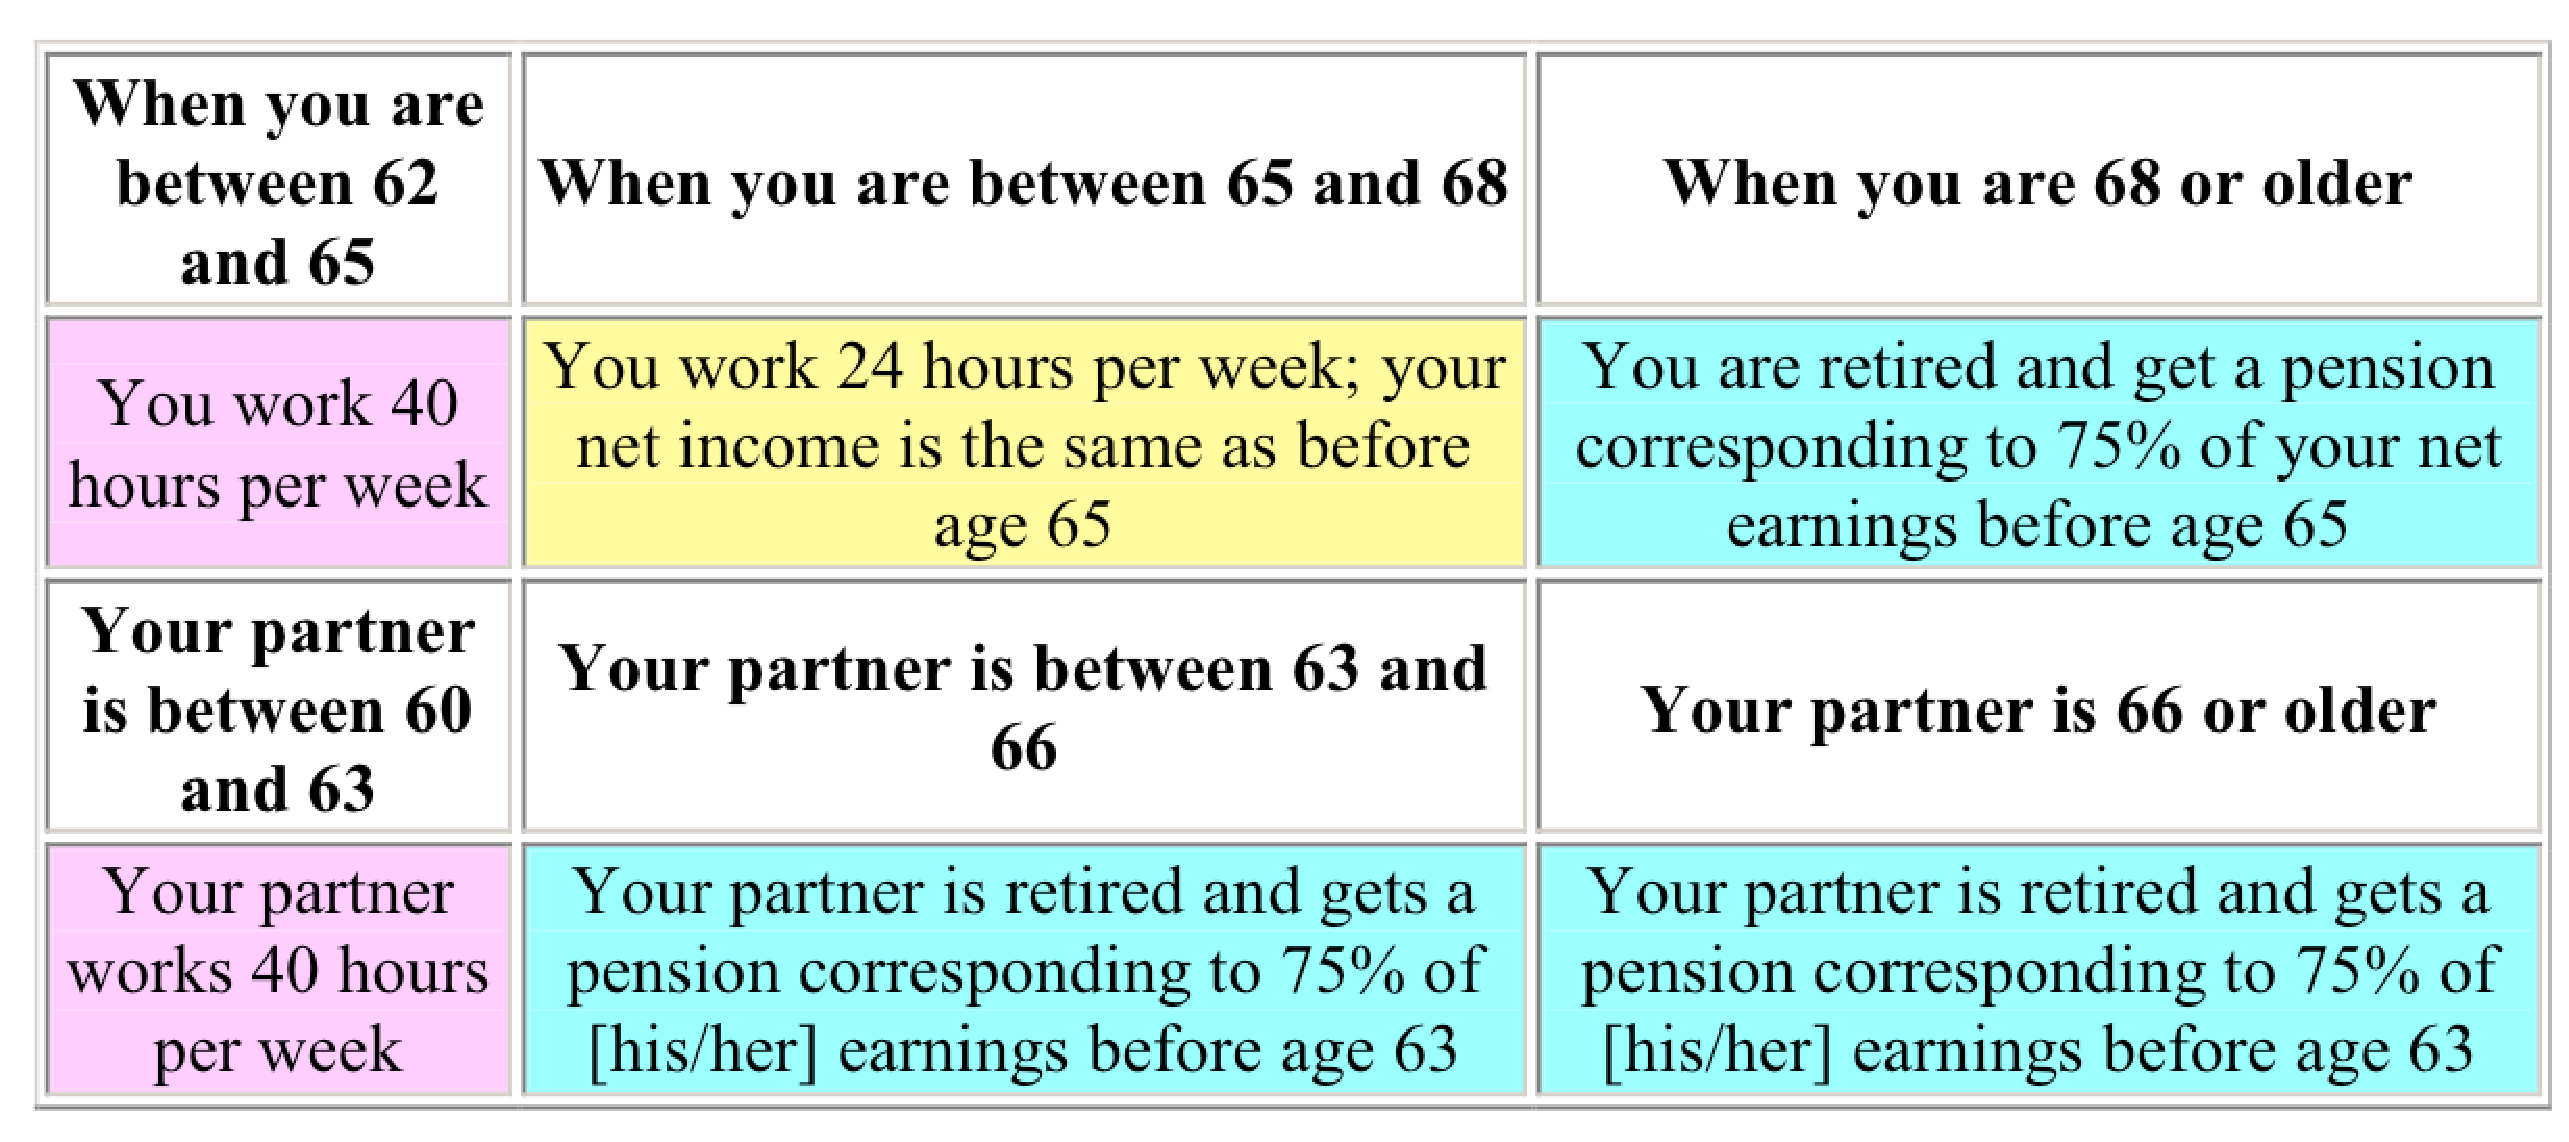
\includegraphics[scale=0.3]{figures/screen.eps}
\caption{\textbf{Screen Shot of Stated-preference Scenario}}
\label{fig:screenshot}
\end{figure}

\begin{figure}[!htbp]
\centering
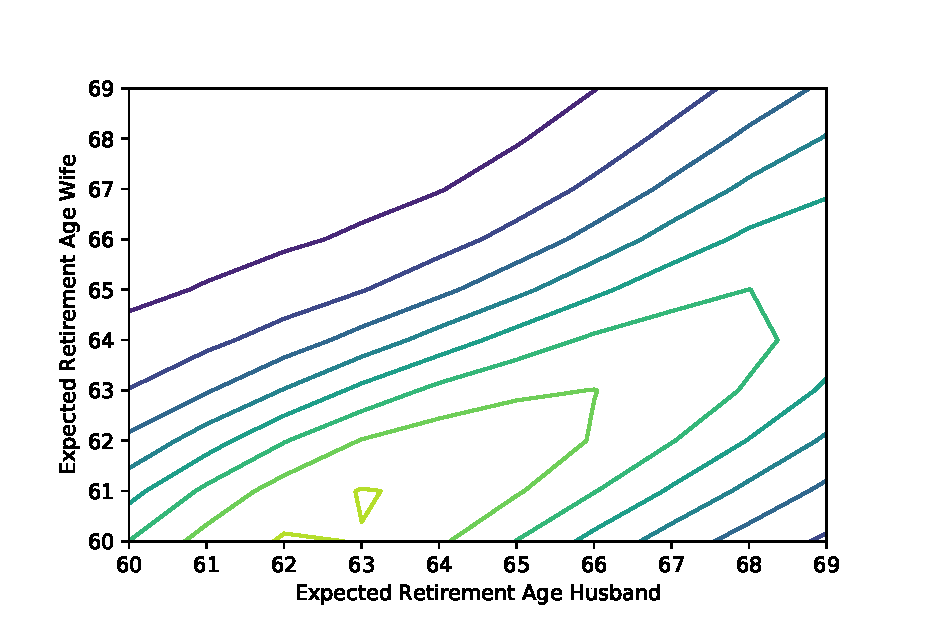
\includegraphics[scale=0.75]{figures/retages.eps}
\caption{\textbf{Simulated Distribution of Retirement Ages, Baseline Model}}
\label{fig:retages}
\end{figure}


\begin{figure}[!htbp]
\centering
\subfloat[Males]{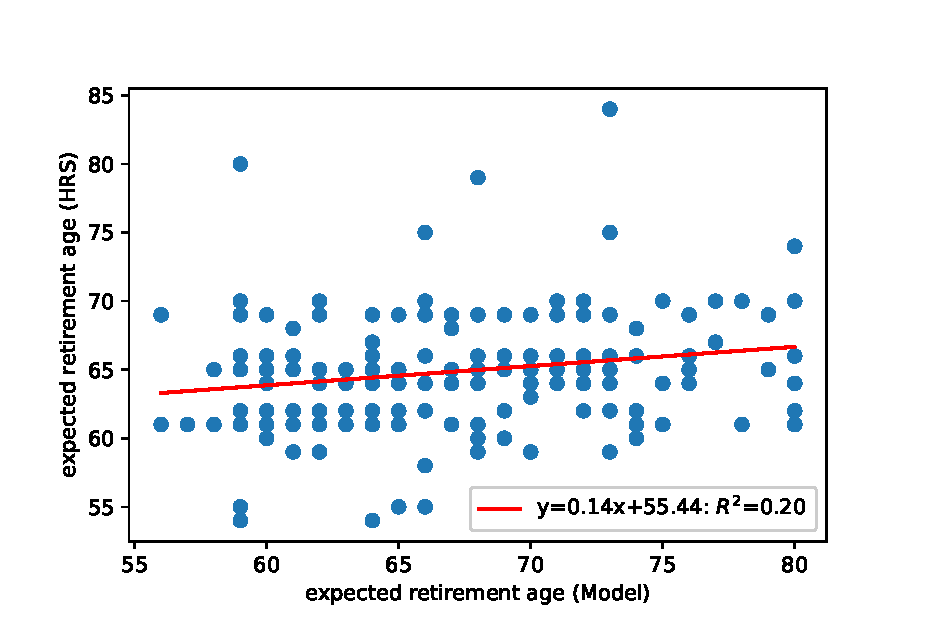
\includegraphics[scale=0.6]{figures/match_males.eps}}
\subfloat[Females]{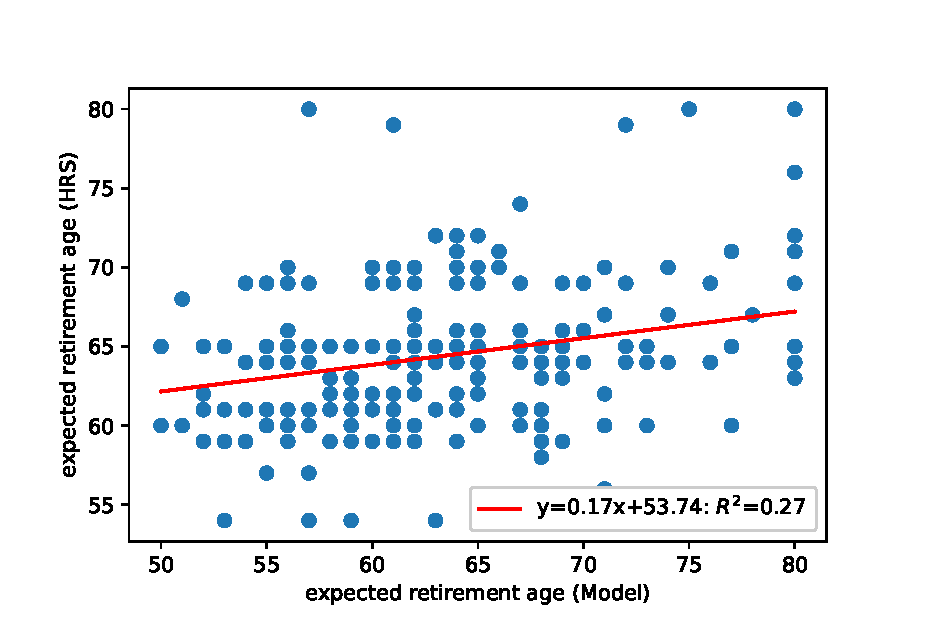
\includegraphics[scale=0.6]{figures/match_females.eps}}
\caption{\textbf{Simulated Retirement Ages and Expected Retirement Ages in HRS}}
\label{fig:match}
\end{figure}

\begin{figure}[!htbp]
\centering
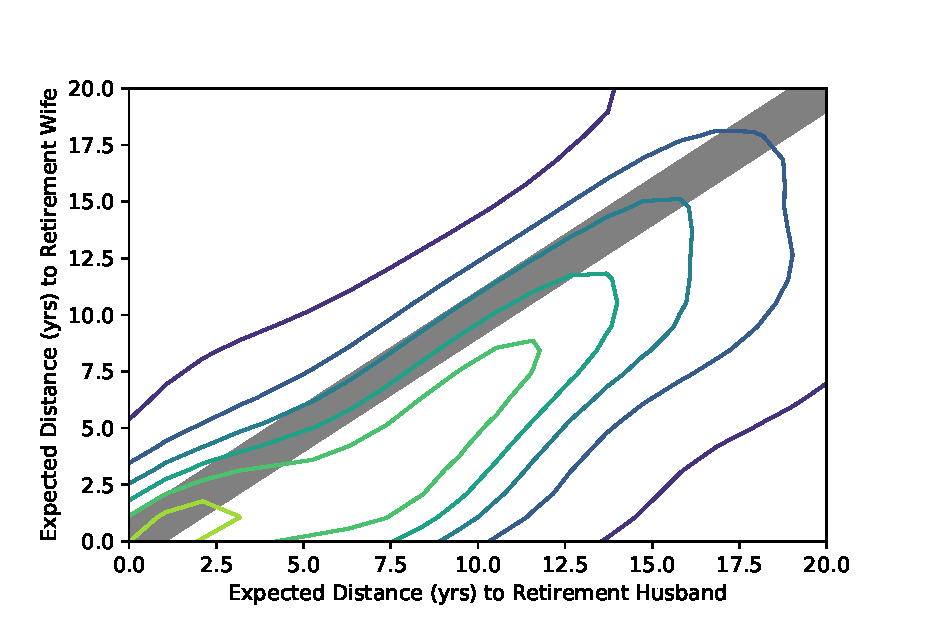
\includegraphics[scale=0.75]{figures/distances.eps}
\caption{\textbf{Distribution of Simulated Distance to Retirement Husbands and Wives}: Shaded area represents distances that are at most one 1 year apart.}
\label{fig:distances}
\end{figure}

\begin{figure}[!htbp]
\centering
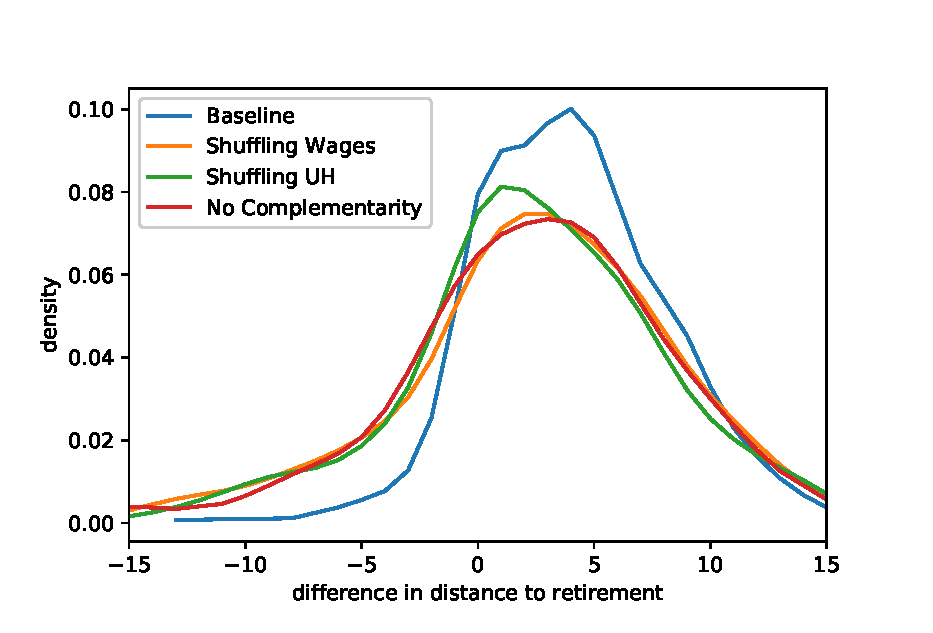
\includegraphics[scale=0.75]{figures/compare_distances.eps}
\caption{\textbf{Simulated Distributions of Difference between Timing of Retirement of Husband and Wife}.}
\label{fig:compare}
\end{figure}

\clearpage
\section*{Tables}


\begin{table}[!htbp]
\centering
{
\def\sym#1{\ifmmode^{#1}\else\(^{#1}\)\fi}
\begin{tabular}{l*{2}{cc}}
\hline\hline
                    &\multicolumn{2}{c}{husbands}&\multicolumn{2}{c}{wives}\\
                    &        mean&          sd&        mean&          sd\\
\hline
age                 &       54.54&        4.49&       56.38&        4.18\\
any health limitations&        0.09&        0.28&        0.07&        0.25\\
college educated    &        0.42&        0.49&        0.44&        0.50\\
job satisfaction    &        0.75&        0.43&        0.75&        0.43\\
hourly wage         &       25.22&       53.69&       31.07&       31.81\\
prov lives to 75 (relative to life-table)&        0.93&        0.25&        0.97&        0.32\\
probability has health limitations at age 62&        0.39&        0.26&        0.40&        0.27\\
\hline
Observations        &         604&            &         604&            \\
\hline\hline
\end{tabular}
}

\caption{\textbf{Summary Statistics Explanatory Variables}: Missing wages are imputed using OLS predictions from previous wages, age and education. Job satisfaction determined using whether respondent is satisfied or very satisfied with job. Subjective survival probabilities to age 75 reported as a ratio of the life-table probability by age and sex.}
\label{tab:sumstats}
\end{table}

\begin{table}[!htbp]
\centering
\begin{tabular}{cccrrrrr}
\hline \hline
& \multicolumn{2}{c}{Retirement Age} & & & & & \\
Scenario & Male & Female & G1    & G2    & G3    & G4    & G5 \\
\hline
1 & 65    & 68    & 50 60 & 55 65 & 60 70 & 65 75 & 70 80 \\
2 & 62    & 65    & 40 40 & 45 45 & 50 50 & 55 55 & 60 60 \\
3 & 68    & 68    & 60 50 & 65 55 & 70 60 & 75 65 & 80 70 \\
4 & 62 (P) 65 & 65    & 50 40 & 55 45 & 60 50 & 65 55 & 70 60 \\
5 & 68    & 65 (P) 68 & 70 60 & 75 65 & 80 70 & 85 75 & 90 80 \\
6 & 65    & 65    & 50 50 & 55 55 & 60 60 & 65 65 & 70 70 \\
\hline \hline
\end{tabular}%
\caption{\textbf{Description of Retirement Scenarios in SP Questions by Randomized Group using an Example}: In Scenario 4 and 5, P refers to partial retirement. If the respondents or the spouses partially retire, their disposable incomes do not change. Their working hours reduce by 40 percent. Respondents were randomly assigned to one of the five groups $G_{1},G_{2},G_{3},G_{4},G_{5}$, with different replacement rates in all scenarios. The first element in each group column gives the RR of the respondent while the second gives the RR of the spouse. }
\label{tab:example}
\end{table}

\clearpage


\begin{table}[!htbp]
\centering
\begin{tabular}{lrrrrrr} 
\hline \hline 
 & \multicolumn{3}{c}{Males} & \multicolumn{3}{c}{Females} \\
\hline
Made for & Scenario 2 & Scenario 4 & Skipped & Scenario 2 & Scenario 4 & Skipped \\
 Males &   0.324 &   0.568 &   0.108 &   0.296 &   0.632 &   0.071 \\ 
 Females &   0.367 &   0.512 &   0.120 &   0.357 &   0.564 &   0.079 \\ 
 Both &   0.349 &   0.531 &   0.120 &   0.296 &   0.629 &   0.075 \\ 
 & Scenario 5 & Scenario 2 & Skipped & Scenario 5 & Scenario 2 & Skipped \\
 Males &   0.454 &   0.420 &   0.127 &   0.518 &   0.389 &   0.093 \\ 
 Females &   0.469 &   0.401 &   0.130 &   0.471 &   0.436 &   0.093 \\ 
 Both &   0.478 &   0.392 &   0.130 &   0.511 &   0.400 &   0.089 \\ 
 & Scenario 3 & Scenario 6 & Skipped & Scenario 3 & Scenario 6 & Skipped \\
 Males &   0.293 &   0.571 &   0.136 &   0.425 &   0.493 &   0.082 \\ 
 Females &   0.312 &   0.534 &   0.154 &   0.436 &   0.479 &   0.086 \\ 
 Both &   0.306 &   0.549 &   0.145 &   0.443 &   0.464 &   0.093 \\ 
\hline \hline 
\end{tabular}

\caption{\textbf{Proportion of Choices Made by Males and Females}: Fraction of respondents (column) who have chosen a particular scenario (three choice situations) for either one of the spouses, or both (rows). In the first choice situation, respondents chose between scenarios 2 and 4 (they could skip), the second, between scenarios 5 and 2 and finally in the third, between scenarios 3 and 6.}
\label{tab:choices}
\end{table}


\begin{table}[!htbp]
\centering
\begin{tabular}{lcc} 
\hline\hline 
 & Males & Females \\ 
Own leisure & $\alpha_{i}^{m}$ & $\beta_{i}^{f}$ \\ 
constant & -1.691 & -0.519 \\ 
 & (0.435) & (0.373) \\ 
age & 0.374 & 0.398 \\ 
 & (0.061) & (0.079) \\ 
health limitations & 1.161 & 0.906 \\ 
 & (0.492) & (0.498) \\ 
college & -0.119 & -0.151 \\ 
 & (0.252) & (0.233) \\ 
spouse responded & 0.142 & 1.431 \\ 
 & (0.361) & (0.432) \\ 
satisfied job & 0.170 & 0.067 \\ 
 & (0.330) & (0.250) \\ 
leisure spouse & 0.209 & 0.086 \\ 
 & (0.043) & (0.035) \\ 
Consumption & $\alpha^{c}$ & $\beta^{c}$ \\ 
 & 0.211 & 0.147 \\ 
 & (0.049) & (0.047) \\ 
Discount factors & $\rho^m$ & $\rho^f$ \\ 
 & 1.026 & 1.020 \\ 
 & (0.010) & (0.012) \\ 
Weights & $\lambda$ &  \\ 
Constant & 0.255 &  \\ 
 & 0.665 &  \\ 
$\log(\frac{w_m}{w_f})$ & 1.508 &  \\ 
 & 1.138 &  \\ 
Heterogeneity & $\eta_i^m$ & $\nu_i^f$ \\ 
Std.Dev & 0.162 & 0.022 \\ 
Correlation & 0.770 &  \\ 
Heterogeneity & $\zeta_i^m$ & $\zeta_i^f$ \\ 
Std.Dev & 0.420 & 0.313 \\ 
Correlation & 1.000 &  \\ 
Heterogeneity & $\rho_i^m$ & $\rho_i^f$ \\ 
Std.Dev & 0.000 & 0.000 \\ 
Correlation & nan &  \\ 
\hline 
$\log L$ & -2594.0 & \\ 
\hline \hline 
\end{tabular} 

\caption{\textbf{Parameter Estimates}: Maximum likelihood estimates and standard errors for the collective model with subjective survival expectations.}
\end{table}


\begin{table}[!htbp]
\centering
\begin{tabular}{lrr}
\toprule
{} & Loglikehood Value & LR Statistic \\
\midrule
Baseline                 &         -2612.816 &        0.000 \\
Fixed Discount Rates (2) &         -2649.015 &       72.398 \\
No Correlation UH (1)    &         -2826.765 &      427.897 \\
No Complementarity (2)   &         -3834.665 &     2443.699 \\
Unitary (1)              &         -5985.378 &     6745.123 \\
\bottomrule
\end{tabular}

\caption{\textbf{Loglikelihood Ratio Test Statistics for Restricted Models}: number of restrictions in parenthesis. The critical value at the 5\% level for 1 restriction is 3.84 and 5.99 for two restrictions.}
\end{table}




\begin{table}[!htbp]
\centering
\begin{tabular}{lrrr}
\toprule
{} & Ret Age Males & Ret Age Females & Fraction Joint \\
\midrule
Baseline           &        65.731 &          63.832 &          0.336 \\
Shuffling Wages    &        65.638 &          63.802 &          0.366 \\
Shuffling UH       &        65.765 &          63.892 &          0.177 \\
No Complementarity &        66.142 &          64.468 &          0.304 \\
\bottomrule
\end{tabular}

\caption{\textbf{Simulated Retirement Ages and Fraction Retiring at Most One Year from Each Other: Explaining Joint Retirement}}
\label{tab:joint}
\end{table}

\begin{table}[!htbp]
\centering
\begin{tabular}{lrrr}
\toprule
{} & Ret Age Males & Ret Age Females & Fraction Retiring Jointly \\
\midrule
Baseline        &        66.744 &          63.657 &                     0.287 \\
No Penalty      &        64.323 &          61.834 &                     0.323 \\
High Penalty    &        67.696 &          64.334 &                     0.228 \\
Low Generosity  &        67.287 &          64.002 &                     0.222 \\
High Generosity &        66.315 &          63.425 &                     0.306 \\
\bottomrule
\end{tabular}

\caption{\textbf{Simulated Retirement Ages and Fraction Retiring at Most One Year from Each Other: Financial Incentives}: The High Penality scenario refers to an Actuarial Reduction Factor of 9\% and Delayed Retirement Credit of 11\% (compared to 6\% and 8\% in the baseline). The low generosity scenario refers to a replacement rate of 40\% while the high generosity scenario refers to a replacement rate of 80\%}
\label{tab:policy}
\end{table}


\clearpage

\section{Appendix: Estimation Results Alternative Specifications}

\begin{table}[!htbp]
\centering
\begin{tabular}{lcc} 
\hline\hline 
 & Males & Females \\ 
Own leisure & $\alpha_{i}^{m}$ & $\beta_{i}^{f}$ \\ 
constant & -1.712 & -0.397 \\ 
 & (0.946) & (0.923) \\ 
age & 0.416 & 0.464 \\ 
 & (0.076) & (0.083) \\ 
health limitations & 1.192 & 1.041 \\ 
 & (0.575) & (0.553) \\ 
college & -0.064 & -0.193 \\ 
 & (0.300) & (0.267) \\ 
spouse responded & 0.317 & 1.677 \\ 
 & (0.445) & (0.480) \\ 
satisfied job & 0.127 & 0.041 \\ 
 & (0.402) & (0.289) \\ 
leisure spouse & -0.474 & -0.437 \\ 
 & (0.064) & (0.060) \\ 
Consumption & $\alpha^{c}$ & $\beta^{c}$ \\ 
 & 0.342 & 0.221 \\ 
 & (0.026) & (0.019) \\ 
Discount factors & $\rho^m$ & $\rho^f$ \\ 
 & 1.000 & 1.000 \\ 
 & (0.000) & (0.000) \\ 
Weights & $\lambda$ &  \\ 
Constant & 0.169 &  \\ 
 & 0.700 &  \\ 
$\log(\frac{w_m}{w_f})$ & 1.768 &  \\ 
 & 1.409 &  \\ 
Heterogeneity & $\eta_i^m$ & $\nu_i^f$ \\ 
Std.Dev & 0.545 & 0.174 \\ 
Correlation & -0.435 &  \\ 
\hline 
$\log L$ & -2617.4 & \\ 
\hline \hline 
\end{tabular} 

\caption{\textbf{Parameter Estimates with Fixed Discount Factors}: Maximum likelihood estimates and standard errors for the collective model with subjective survival expectations.}
\end{table}

\clearpage

\begin{table}[!htbp]
\centering
\begin{tabular}{lcc} 
\hline\hline 
 & Males & Females \\ 
Own leisure & $\alpha_{i}^{m}$ & $\beta_{i}^{f}$ \\ 
constant & 1.322 & -2.914 \\ 
 & (0.387) & (0.591) \\ 
age & 0.338 & 0.427 \\ 
 & (0.049) & (0.084) \\ 
health limitations & 0.899 & 1.232 \\ 
 & (0.380) & (0.431) \\ 
college & 0.376 & -0.174 \\ 
 & (0.209) & (0.214) \\ 
spouse responded & 0.248 & 0.658 \\ 
 & (0.261) & (0.368) \\ 
satisfied job & -0.096 & 0.027 \\ 
 & (0.234) & (0.244) \\ 
leisure spouse & -0.174 & -0.252 \\ 
 & (0.033) & (0.050) \\ 
Consumption & $\alpha^{c}$ & $\beta^{c}$ \\ 
 & 0.086 & 0.123 \\ 
 & (0.024) & (0.041) \\ 
Discount factors & $\rho^m$ & $\rho^f$ \\ 
 & 1.059 & 1.021 \\ 
 & (0.010) & (0.012) \\ 
Weights & $\lambda$ &  \\ 
Constant & 0.191 &  \\ 
 & 0.303 &  \\ 
$\log(\frac{w_m}{w_f})$ & 0.380 &  \\ 
 & 0.337 &  \\ 
Heterogeneity & $\eta_i^m$ & $\nu_i^f$ \\ 
Std.Dev & 5.563 & 4.288 \\ 
Correlation & 0.000 &  \\ 
\hline 
$\log L$ & -2826.8 & \\ 
\hline \hline 
\end{tabular} 

\caption{\textbf{Parameter Estimates without Correlation in Unobserved Heterogeneity}: Maximum likelihood estimates and standard errors for the collective model.}
\end{table}

\clearpage


\begin{table}[!htbp]
\centering
\begin{tabular}{lcc} 
\hline\hline 
 & Males & Females \\ 
Own leisure & $\alpha_{i}^{m}$ & $\beta_{i}^{f}$ \\ 
constant & -1.263 & -0.339 \\ 
 & (0.446) & (0.312) \\ 
age & 0.451 & 0.457 \\ 
 & (0.067) & (0.081) \\ 
health limitations & 1.202 & 1.042 \\ 
 & (0.544) & (0.453) \\ 
college & 0.064 & -0.181 \\ 
 & (0.270) & (0.213) \\ 
spouse responded & 0.679 & 1.071 \\ 
 & (0.328) & (0.316) \\ 
satisfied job & 0.018 & -0.192 \\ 
 & (0.322) & (0.236) \\ 
leisure spouse & 0.000 & 0.000 \\ 
 & (0.000) & (0.000) \\ 
Consumption & $\alpha^{c}$ & $\beta^{c}$ \\ 
 & 0.062 & 0.066 \\ 
 & (0.020) & (0.021) \\ 
Discount factors & $\rho^m$ & $\rho^f$ \\ 
 & 1.049 & 1.029 \\ 
 & (0.012) & (0.013) \\ 
Weights & $\lambda$ &  \\ 
Constant & -0.057 &  \\ 
 & 0.320 &  \\ 
$\log(\frac{w_m}{w_f})$ & 0.515 &  \\ 
 & 0.287 &  \\ 
Heterogeneity & $\eta_i^m$ & $\nu_i^f$ \\ 
Std.Dev & 2.425 & 1.685 \\ 
Correlation & 0.997 &  \\ 
Heterogeneity & $\zeta_i^m$ & $\zeta_i^f$ \\ 
Std.Dev & 0.000 & 0.000 \\ 
Correlation & nan &  \\ 
\hline 
$\log L$ & -2849.3 & \\ 
\hline \hline 
\end{tabular} 

\caption{\textbf{Parameter Estimates without Complementarity in Leisure}: Maximum likelihood estimates and standard errors for the collective model.}
\end{table}

\clearpage

\begin{table}[!htbp]
\centering
\begin{tabular}{lcc} 
\hline\hline 
 & Males & Females \\ 
Own leisure & $\alpha_{i}^{m}$ & $\beta_{i}^{f}$ \\ 
constant & -2.343 & -1.485 \\ 
 & (105.087) & (26.932) \\ 
age & 0.338 & 0.524 \\ 
 & (nan) & (nan) \\ 
health limitations & 2.522 & 2.046 \\ 
 & (nan) & (nan) \\ 
college & -0.042 & 0.126 \\ 
 & (nan) & (12.078) \\ 
spouse responded & 0.531 & 1.367 \\ 
 & (nan) & (nan) \\ 
satisfied job & 0.408 & 0.147 \\ 
 & (25.050) & (10.634) \\ 
leisure spouse & 0.550 & 0.480 \\ 
 & (nan) & (nan) \\ 
Consumption & $\alpha^{c}$ & $\beta^{c}$ \\ 
 & 0.196 & 0.135 \\ 
 & (446.147) & (167.942) \\ 
Discount factors & $\rho^m$ & $\rho^f$ \\ 
 & 1.019 & 1.018 \\ 
 & (128.992) & (nan) \\ 
Weights & $\lambda$ &  \\ 
Constant & 5.531 &  \\ 
 & 0.000 &  \\ 
$\log(\frac{w_m}{w_f})$ & 0.000 &  \\ 
 & 0.000 &  \\ 
Heterogeneity & $\eta_i^m$ & $\nu_i^f$ \\ 
Std.Dev & 0.000 & 0.000 \\ 
Correlation & nan &  \\ 
\hline 
$\log L$ & -5985.4 & \\ 
\hline \hline 
\end{tabular} 

\caption{\textbf{Parameter Estimates of Unitary Model}: Maximum likelihood estimates and standard errors}
\end{table}

\end{document}


\clearpage

\begin{table}[!htbp]
\centering
% Table generated by Excel2LaTeX from sheet 'Sheet1'
\begin{tabular}{|c|c|c|c|c|c|c|c|c|c|c|c|}
\hline
                &              60 &              61 &              62 &              63 &              64 &              65 &              66 &              67 &              68 &              69 &              70 \\
                \hline

             60 &   $\bullet$              &                 &                 &                 &                 &                 &                 &                 &                 &                 &                 \\\hline

             61 &                 &    $\bullet$              &                 &                 &                 &                 &                 &                 &                 &                 &                 \\\hline

             62 &                 &                 &    $\bullet$              &                 &                 &                 &                 &                 &                 &                 &                 \\\hline

             63 &                 &                 &                 &    $\bullet$              &                 &                 &                 &                 &                 &                 &                 \\\hline

             64 &                 &                 &                 &                 &   $\bullet$               &                 &                 &                 &                 &                 &                 \\\hline

             65 &   $\Box$              &                 &                 &                 &               &      $\bullet$               &                &                 &                 &                 &                 \\\hline

             66 &                 &  $ \Box$              &                 &                 &                 &                 &   $\bullet$                 &               &                 &                 &                 \\\hline

             67 &                 &                 &   $\Box$              &                 &                 &                 &                 &  $\bullet$               &                 &                 &                 \\\hline

             68 &                 &                 &                 &    $\Box$              &                 &                 &                 &                 &   $\bullet$              &                 &                 \\\hline

             69 &                 &                 &                 &                 &   $\Box$               &                 &                 &                 &                 &      $\bullet$           &                 \\\hline

             70 &                 &                 &                 &                 &                 &     $\Box$             &                 &                 &                 &                 &   $\bullet$              \\\hline

\end{tabular}
\caption{\textbf{Joint Retirement Patterns}: The horizontal axis indicates the retirement age of male, the vertical axis indicates the retirement age of female. In total, we have 11*11=121 potential realizations. Each cell in the table indicates one outcome.}
\label{tab:jointpatterns}
\end{table}

\begin{table}[!htbp]
\centering
\begin{tabular}{lcc} 
\hline\hline 
 & Males & Females \\ 
Own leisure & $\alpha_{i}^{m}$ & $\beta_{i}^{f}$ \\ 
constant & -1.045 & -0.384 \\ 
 & (0.535) & (0.660) \\ 
age & 0.295 & 0.337 \\ 
 & (0.055) & (0.074) \\ 
health limitations & 0.760 & 0.712 \\ 
 & (0.369) & (0.411) \\ 
college & -0.026 & -0.109 \\ 
 & (0.184) & (0.198) \\ 
spouse responded & 0.172 & 1.185 \\ 
 & (0.272) & (0.371) \\ 
satisfied job & 0.151 & 0.075 \\ 
 & (0.240) & (0.213) \\ 
leisure spouse & -0.328 & -0.353 \\ 
 & (0.048) & (0.055) \\ 
Consumption & $\alpha^{c}$ & $\beta^{c}$ \\ 
 & 0.054 & 0.067 \\ 
 & (0.018) & (0.025) \\ 
Discount factors & $\rho^m$ & $\rho^f$ \\ 
 & 1.040 & 1.025 \\ 
 & (0.011) & (0.012) \\ 
Weights & $\lambda$ &  \\ 
Constant & 0.321 &  \\ 
 & 0.800 &  \\ 
$\log(\frac{w_m}{w_f})$ & 1.695 &  \\ 
 & 1.410 &  \\ 
Heterogeneity & $\eta_i^m$ & $\nu_i^f$ \\ 
Std.Dev & 0.714 & 0.095 \\ 
Correlation & -0.999 &  \\ 
Heterogeneity & $\zeta_i^m$ & $\zeta_i^f$ \\ 
Std.Dev & 0.960 & 0.834 \\ 
Correlation & 1.000 &  \\ 
\hline 
$\log L$ & -2607.0 & \\ 
\hline \hline 
\end{tabular} 

\caption{\textbf{Parameter Estimates without Survival Probabilities}: Maximum likelihood estimates and standard errors for the collective model.}
\end{table} 